In our era technology has a foundamental role in almost every field. From the simple communications activities to those related to medical researches, technology is something we cannot do without. It is also a great opportunity in educational field, where it is demonstrated that the so called "stealth learning" (i.e. the help of technologies in educational scope) \cite{Sharp} is a solution to create a greater emotional involvement and that has as a consequence the ability to increase learner's learning opportunities. In our specific case, stealth learning is suitable for the treatment of patients affected by NDD to develop their cognitive, emotional and intellectual skills.
\section{Modern technologies for NDD people}
All the new existing technologies are now helping therapists and families to deal with neurological disabilities. In fact, in addition to virtual reality, smart objects, multisensor environments or smart spaces and conversational agents are used.\\
Smart objects are devices that can interact not only with the user but also with other similar devices and with the surrounding environment. Physical world can be described in terms of three properties \cite{Smart}: awareness (is a smart object to be able to understand events and human activities occurring in the physical world), representation (refers to a smart object's application and programming model) and interaction (denotes the object's ability to converse with the user in terms of input, output, control, and feedback).\\
Examples are Dolphin Sam \cite{Dolphin} and  Huggable \cite{Huggable}. \\
Smart spaces or multisensor environments are rooms in which children can play or interact in a controlled way because they are equipped with techonological items like cameras, smart objects, leds and projectors.
\\
Examples are Magic K room e M4All \cite{M4all}. \\
Conversational agents are devices that can communicate with the user in a manner consistent with what is required: an interaction of the user is answered by the agent who must be with sense.\\
\begin{figure}[H]
\centering
\begin{minipage}[c]{.40\textwidth}
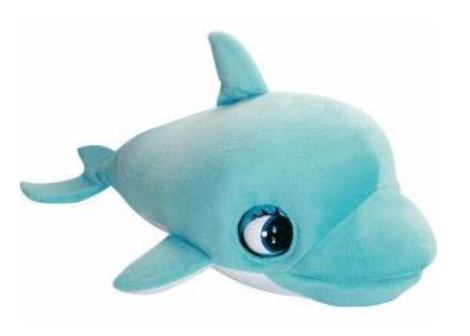
\includegraphics[width=1\textwidth]{immagini/delfino.png}
\end{minipage}%
\hspace{10mm}%
\begin{minipage}[c]{.40\textwidth}
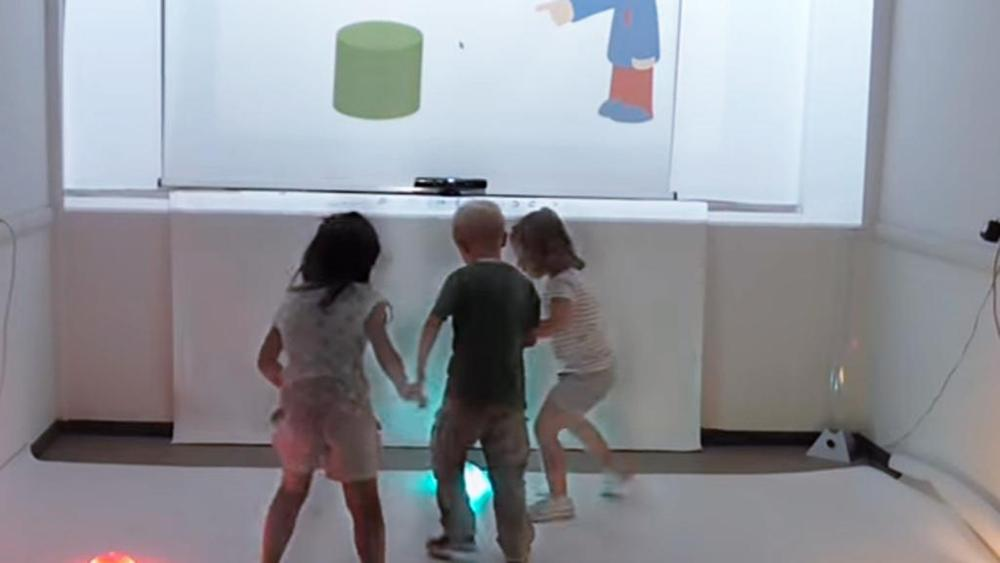
\includegraphics[width=1\textwidth]{immagini/stanzamagica.jpg}
\end{minipage}
\caption{Dolphin Sam and Magic K Room}\label{fig:smartimages}
\end{figure}
\section{Virtual Reality}
\section{Touchscreen}
\section{Google Chromecast}
\section{Projects about food education}

